\section{Effiziente Berechnung der CWT}
\rhead{Berechnung der CWT}

Betrachten wir zuerst die folgende Gleichung
\begin{equation}
\mathcal{W}f (a,b)
=
\langle f,\psi_{a,b}\rangle
=
\frac{1}{\sqrt{|a|}}\int_{-\infty}^\infty f(t)\,
	\overline{\psi\left(\frac{t-b}{a}\right)}\,\mathrm{d}t,\label{complex:CWT}
\end{equation}
welche in Definition~\ref{cwt:definition} die kontinuierliche Wavelet-Transformation definierte.
Dieses Integral entspricht der Faltung zwischen $f(t)$ und 
\begin{equation} 
    g(t) 
    = \frac{1}{\sqrt{|a|}} \overline{\psi\left(\frac{-t}{a}\right)} \,.
\end{equation}
Der Standard-Trick zur effizienten Berechnung einer Faltung ist die Multiplikation im Frequenzbereich.
\begin{equation} 
\mathcal{W}f (a,b) = (f*g)(t) = \mathcal{F}^{-1}\left\lbrace\hat f(\omega) \hat g (\omega) \right\rbrace.
\end{equation}
Dafür benötigen wir die Fouriertransformierte $\hat g (\omega)$:
\begin{align*}
	\hat g (\omega) = 
    \mathcal{F}\left\lbrace \frac{1}{\sqrt{|a|}} \overline{\psi\left(\frac{-t}{a}\right)}\right\rbrace 
	&= \frac{1}{\sqrt{|a|}} \int_{-\infty}^{\infty}\overline{\psi\left(\frac{-t}{a}\right)}\,e^{-i\omega t}\,\mathrm{d}t\\
	&= \frac{1}{\sqrt{|a|}} \overline{\int_{-\infty}^{\infty}\psi\left(\frac{-t}{a}\right)e^{i\omega t}\,\mathrm{d}t}  
    & \left(\text{Subst. } t' = \frac{-t}{a}\right)\\
	&= \frac{1}{\sqrt{|a|}} \overline{\int_{-\infty}^{\infty}\psi\left(t'\right)e^{-ia\omega t'} |a|\,\mathrm{d}t'}\\
	&= \sqrt{|a|} \, \overline{\hat{\psi}\left(a\omega\right)}.
\end{align*}
Gleichung~\eqref{complex:CWT} lässt sich somit schreiben als
\begin{equation}
\mathcal{W}f(a,b)
= \mathcal{F}^{-1}\left\lbrace\hat{f}(\omega) \sqrt{|a|}\, \overline{\hat{\psi}\left(a\omega\right)}\right\rbrace. \label{complex:fcwt}
\end{equation}

Mittels Fourier-Transformation lässt sich die Wavelet-Transformation folglich besonders elegant berechnen.
Kontinuierliche Funktionen sind für numerische Systeme jedoch ungeeignet.
Die CWT muss in $a$ und $b$ diskretisiert werden.
Die Diskretisierung von $b$ entspricht vorteilhaft gerade derjenigen des Signals selbst.
Dann lässt sich die Fourier-Transformation mittels FFT effizient berechnen und Gleichung~\eqref{complex:fcwt} wird zu
\begin{equation}
	\mathcal{W}f(a,b) = \text{IFFT}\left(\text{FFT}(f) \, \overline{\hat{\psi}\left(a\omega\right)}\right)\footnote{Der Faktor $\sqrt{|a|}$ wurde hierbei weggelassen.
		Hierdurch werden die hohen Frequenzen stärker gewichtet und $|\mathcal{W}f(a,b)|$ ist gerade proportional zur Amplitude der analysierten Signalkomponente.
        Zudem erzielen wir im Diskreten nicht exakt die Faltung, sondern die zirkuläre Version davon. 
        Mehr dazu im Abschnitt~\ref{complex:circ-conv-padding}.
	}. \label{complex:ffcwt}
\end{equation}

Diese Gleichung muss für jedes $a$ einzeln gelöst werden.
Sie wird besonders interessant, wenn das Wavelet im Frequenzbereich eine geschlossene, analytische Form besitzt.
Dann benötigt man nur eine FFT für das Signal, so wie für jedes $a$ eine inverse FFT und eine punktweise Multiplikation zwischen Signal und Wavelet.

\subsection{Das Haar-Wavelet}
\begin{figure}
	\centering
	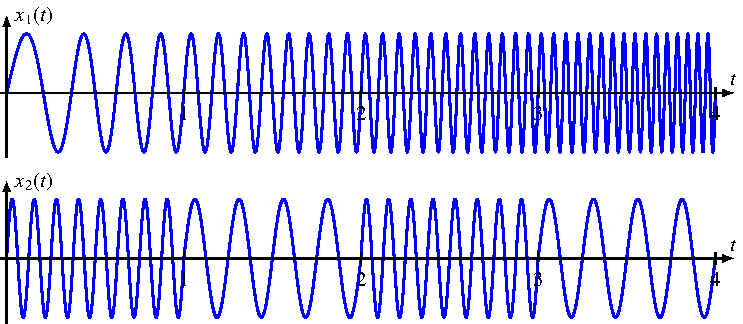
\includegraphics[width=\textwidth, keepaspectratio]{papers/complex/images/signals.pdf}
	\caption{Die beiden Beispielsignale $x_1(t)$ und $x_2(t)$}
\end{figure}
Für ein Beispiel benötigen wir zwei Dinge: ein Wavelet und ein Beispielsignal.
Nehmen wir für den Anfang das einfachste aller Wavelets, das Haar-Wavelet.
Als Signal nehmen wir zwei Sinus-Schwingungen, eine mit linear ansteigender und eine mit stückweise konstanter Frequenz.
\begin{align}
    x_1(t) &= \sin\left( \int_{0}^{t} 2\pi f_1(t')\,\mathrm{d}t'\right) & f_1(t) &= 2 + 6/4 \cdot t \\
    x_2(t) &= \sin\left( \int_{0}^{t} 2\pi f_2(t')\,\mathrm{d}t'\right) & f_2(t) &= \left\lbrace \begin{matrix}
    4, & &t& < 1\\
    8, & 1.0 \le &t& < 2.0\\
    4, & 2.0 \le &t& < 3.0\\
    8, & 3.0 \le &t&\\
    \end{matrix}\right.
\end{align}
Zudem benötigen wir das Haar-Wavelet und seine Fourier-Transformierte.
In diesem Abschnitt sei das Wavelet zentriert um $t=0$.
Die daraus resultierende Symmetrie wird sich in der Berechnung der Fourier-Transformation als hilfreich erweisen.

\begin{definition}
	\label{complex:def-haar-wavelet}
	Das zentrierte, reelle Haar-Wavelet besitzt folgende Gestalt:
	\[
	\psi_{\text{Haar}}(t) = \left\lbrace\begin{matrix*}[r]
	1 & -\frac{1}{2} \le t < 0  \\
	-1 & 0 \le t < \frac{1}{2} \\
	0 & \text{sonst}.
	\end{matrix*} \right.\label{complex:def-haar}
	\]
\end{definition}
Die Fourier-Transformierte von $\psi_{\text{Haar}}$ berechnet sich wie folgt:
\begin{align}
	\mathcal F \psi_\text{Haar}  
	&= \frac{1}{\sqrt{2\pi}}\int_{-\infty}^{\infty} \psi_\text{Haar} e^{-i\omega t} \,\mathrm{d}t\nonumber\\
	&= \frac{1}{\sqrt{2\pi}}\left( \int_{-1/2}^{0} e^{-i\omega t} \,\mathrm{d}t - \int_{0}^{1/2} e^{-i\omega t}\,\mathrm{d}t \right) \nonumber\\
	&= \frac{1i}{\sqrt{2\pi}\omega}\left( \left[ e^{-i\omega t}\right]_{-1/2}^0  - \left[ e^{-i\omega t}\right]_{0}^{1/2} \right)\nonumber\\
	&= \frac{1i}{\sqrt{2\pi}}\left( \frac{1-\cos(\omega/2)}{\omega/2}\right)\label{complex:f-psi-haar}
\end{align}
Das Haar-Wavelet ist also nicht nur im Zeitbereich besonder einfach, sondern auch im Frequenzbereich.
Insbesondere lässt sich die mit $a$ skalierte Version des Wavelets durch Satz~\ref{four-int:trans-dial} direkt im Frequenzbereich berechnen.
Auffallend ist zudem, dass das im Zeitbereich besonders gut lokalisierte Haar-Wavelet in der Frequenz sehr schlecht lokalisiert ist.
$\mathcal{F}\psi_\text{Haar}$ ist in Abbildung \ref{complex:haar} dargestellt.
\begin{figure}
	\centering
	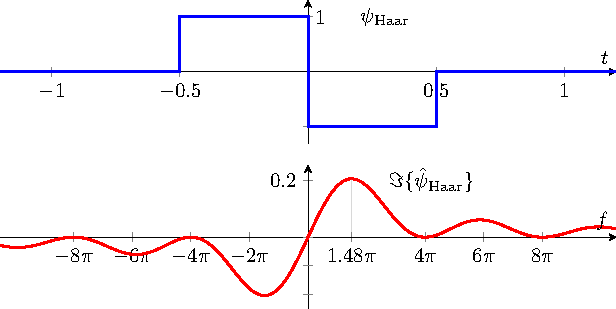
\includegraphics{papers/complex/images/haar.pdf}
	\caption{Das Haar-Wavelet}
	\label{complex:haar}
\end{figure}
\[\hat{\psi}_\text{Haar} = \frac{1i}{2\sqrt{\pi}}\left( \frac{1-\cos(\omega/2)}{\omega/2}\right) \]

\begin{figure}
	\centering
	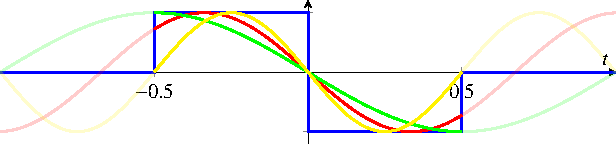
\includegraphics{papers/complex/images/haar_dom.pdf}
	
	\caption{Blau: $\psi_\text{Haar}$, Rot: $\sin ({\color{red}\omega_\psi}\cdot t)$, Gelb: $\sin ({\color{yellow}1.0}\cdot 2\pi t)$, Grün: $\sin ({\color{green}0.5}\cdot 2\pi t)$}
	\label{complex:dom-freq}
\end{figure}
An dieser Stelle definieren wir noch die \emph{Dominante Frequenz} eines Wavelets.
\begin{definition}
	Die Fourier-Transformierte eines Wavelets erreicht den maximalen Betrag bei der \emph{dominante Frequenz $\omega_\psi$}.
	\begin{equation}
		\max_{\omega}\left|\hat\psi(\omega)\right| = \left|\hat\psi(\omega_\psi)\right|
	\end{equation}
	
\end{definition}

Die dominante Frequenz erlaubt es, die $a$-Achse der Wavelet-Transformation als Frequenz-Achse zu interpretieren.
Für die Momentanfrequenz gilt
\begin{align}
	\omega(t) \approx \omega_\psi\,/\,a_\text{max}.
\end{align}
Diese Interpretation ist natürlich nur zulässig, wenn das Signal zum betrachteten Zeitpunkt nur eine dominante Frequenz-Komponente beinhaltet.
Bei unseren Beispielsignalen ist dies der Fall.
Abbildung~\ref{complex:dom-freq} illustriert die Bedeutung von $\omega_\psi$ für das Haar-Wavelet.
Es ist die Frequenz, bei welcher das Skalarprodukt mit dem Wavelet maximal wird.

% Image after gabor wavelet
Somit haben wir für unser Beispiel alles zusammen.
Nach einer Diskretisierung der Variablen überlassen wir die Arbeit dem Computer.
Dies liefert die Bilder aus Abbildung~\ref{complex:haar-ex}.

Wie erwartet ist die Lokalisierung in der Frequenz zimelich schlecht.
Das Haar-Wavelet gibt den Zeitpunkt einer Änderungen der Frequenz zwar sehr genau wieder, die Frequenz selbst ist jedoch kaum ablesbar.
Als Orientierungshilfe sind $a_\text{max} (b) = \max_a{|\Wave x_n(a,b)|}$ weiss hervorgehoben.
Sie weichen um $\omega_\psi$ von der Signal-Frequenz ab, welche als Schwingung in der Amplitude gut erkennbar ist.
Dies werden wir im Abschnitt~\ref{complex:separate} durch komplexe Wavelets vermeiden.
Zuerst kümmern wir uns aber um die Lokalisierung in der Frequenz.
